\documentclass[xcolor={usenames,dvipsnames,svgnames}, compress]{beamer}

% \usepackage[utf8]{inputenc}
\usepackage{booktabs}
\usepackage{dcolumn}
\usepackage{colortbl}
\usepackage{hyperref}
\usepackage[no-math]{fontspec}
\usepackage{ifxetex}
\usepackage{amsmath}
\usepackage{biblatex}


\usetheme{enziteto}

\setbeamertemplate{headline}{}

\begin{document}

% \title{Metodi di Apprendimento Statistico-Relazionale: Sum-Product Network \& Co-clustering}
\title{Iterated Pysoner's Dilemma}
\subtitle{Or how an altruistic behaviour can emerge by iterating selfish games}
\author{antonio vergari - \emph{an irreducible reductionist}}
% \institute{Lacam$@$DIB$@$Uniba}
\institute{Università degli Studi di Bari}
\department{Dipartimento di Informatica}
\laboratory{LACAM}
\group{Machine Learning}
\institutelogo{\includegraphics[width=25pt]{figures/unibaba}}
\lablogo{\includegraphics[width=35pt]{figures/lacam}}

\footnotesize \let\small\footnotesize

{
  \setbeamertemplate{headline}{}
  \setbeamertemplate{footline}{}
  \begin{frame}
    \titlepage
  \end{frame}
}

\section{Context \& Background}
{\setbeamertemplate{headline}{}
  \begin{frame}
    \sectionpage
  \end{frame}
}

\begin{frame}
  \frametitle{ Prisoner's Dilemma}
  The \emph{\textbf{Prisoner's Dilemma}} (\textbf{PD}) is a two-players perfect information game where each player is asked to
  do a single decision: \textbf{C}ooperate or \textbf{D}efect,
  according to a payoff matrix:
  \begin{table}[c]
    \centering
    \begin{tabular}[htbp]{c c c}
      & \textbf{C} & \textbf{D} \\
      \midrule
      \textbf{C} & $(R,R)$ & $(S,T)$ \\
      \midrule
      \textbf{D} & $(T,S)$ & $P,P$ \\
      \bottomrule
    \end{tabular}
  \end{table}\par\bigskip

  for any payoff combination $T > R > P > S$.\par\bigskip

  The Nash equilibrium is $P, P$, the Pareto's one is $R,R$.

  There is no need to simulate
  anything to know a \emph{rational agent strategy}.\par\bigskip


\end{frame}

\begin{frame}
  \frametitle{Iterated Prisoner's Dilemma}
  For $2R > S + T$, the \emph{\textbf{Iterated Prisoner's Dilemma}}
  (\textbf{IPD}) is a sequence of $N$ PD Games.

  Each player's
  outcome is the sum of the $N$ payoffs received.\par\bigskip

  Again, a rational player would always \textbf{D}efect (it can be
  proved inductively this is the dominant strategy).\par\bigskip

  However, some key factors make it differ from a simple PD:
  \begin{itemize}
  \item more than four strategies
  \item possibility to change strategies on new information
    \item evironment (other players strategies) adds variability
  \end{itemize}
\end{frame}

\begin{frame}
  \frametitle{Why and what to simulate}
  While, given the player strategies, one can predict the outcome of a
  single IPD game between two players,
  it is not easy to predict the global outcome of \emph{several IPD games
  amongst
  all players} (it can be computed as the sum of payoffs received
along all games).\par\bigskip


The outcome now depends on the \textbf{payoff matrix}, \textbf{player histories}, and
\textbf{player population }characterization.\par\bigskip 


  Other notions of \emph{bounded rationality} can complicate things
  even more.

  Moreover, remind the notion of Hofstader's
  \emph{superrationality}\par\bigskip

  Following Axelrod's road two kinds of simulations are presented:
  \begin{itemize}
  \item simulating exhaustive pairwise IDP Games for a population of
    players
  \item simulating the evolution of player strategies a fixed size population across generations  
  \end{itemize}
\end{frame}

\section{Modeling}
{\setbeamertemplate{headline}{}
  \begin{frame}
    \sectionpage
  \end{frame}
}

\begin{frame}
  \frametitle{Components}
  \begin{center}
    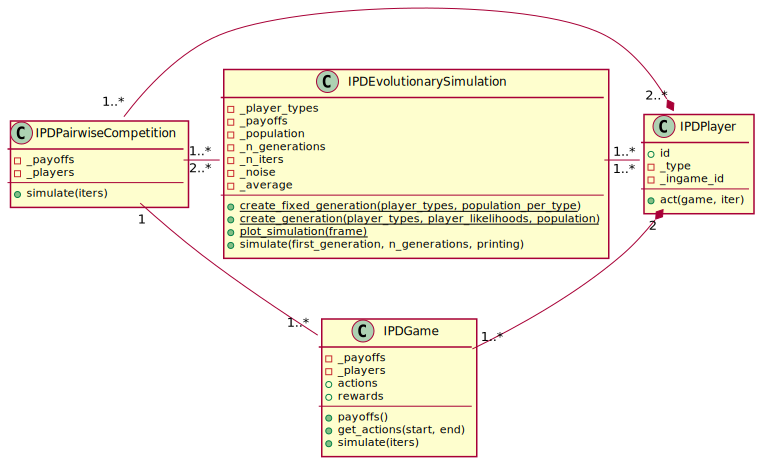
\includegraphics[width=1.0\textwidth]{../uml/class-diagram-full.pdf}
  \end{center}  
\end{frame}

\begin{frame}
  \frametitle{Simulating IDP Game}
  \begin{center}
    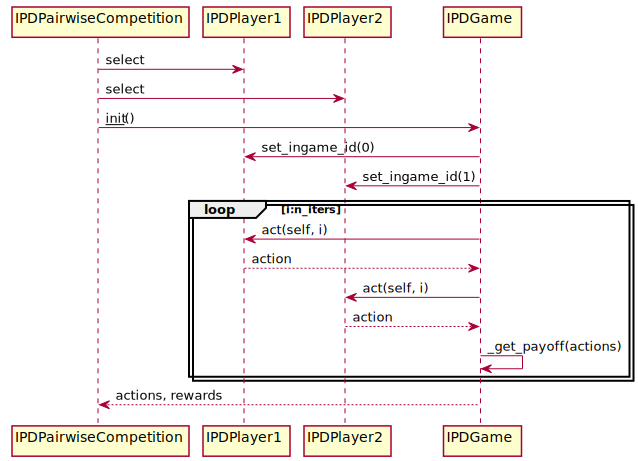
\includegraphics[width=1.0\textwidth]{../uml/sequence-competition.pdf}
  \end{center} 
\end{frame}

\begin{frame}
  \frametitle{Players}
  \begin{center}
    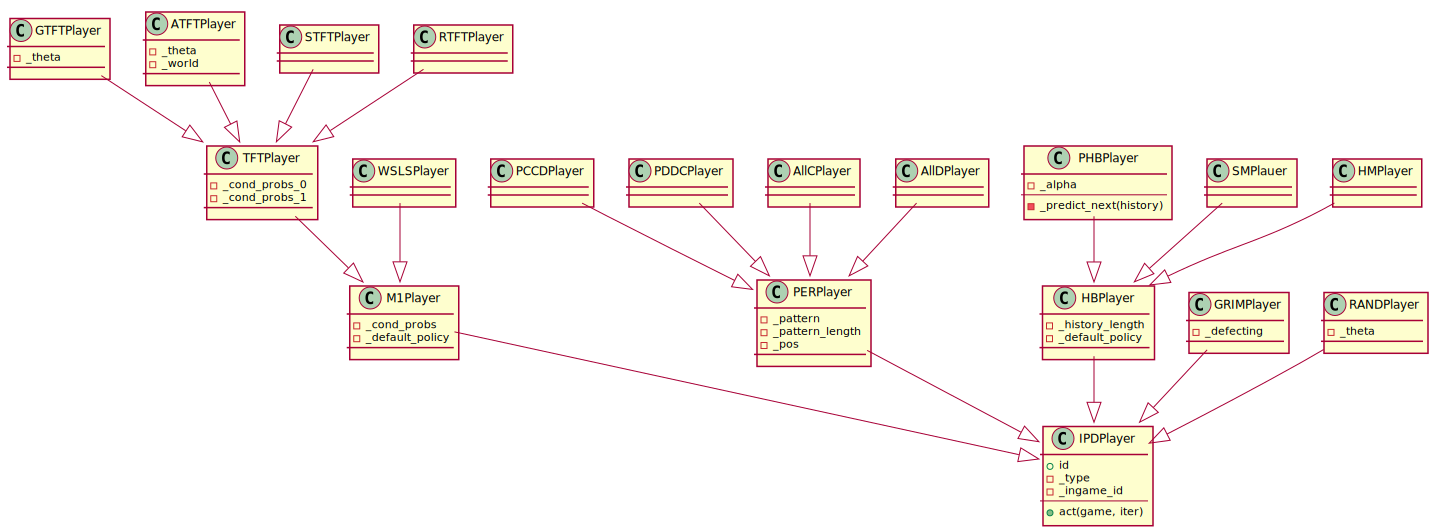
\includegraphics[width=1.0\textwidth]{../uml/all-players.pdf}
  \end{center} 
\end{frame}


\section{Player types}
{\setbeamertemplate{headline}{}
  \begin{frame}
    \sectionpage
  \end{frame}
}

\begin{frame}
  \frametitle{Implementing player strategies}

  Fifteen different concrete agent behaviours have been implemented,
  for a total of ninenteen classes, structured on a generalization
  hierarchy whose root is \textbf{IPDPlayer}.\par\bigskip

  Aggregating by taking into account the ability of to exploit the information about the payoff matrix or the past actions:
  
  \begin{description}
  \item[\textbf{Deterministic and/or periodic}] agents whose decisions
    are fixed or highly predicible.
    They do not take advantage of the history of previous rewards and actions
  \item[\textbf{Memory-1 (stochastic)}] players that are influenced by
    some random variable or probability distribution.
    \emph{Memory-N} agents derive these probabilities from the previous N moves (of both players)
  \item[\textbf{History based}]their decision is highly dependent on the (partial or total) history of the opponent moves
  \end{description}

  Among the not implemented strategies, some noteworthy ones are:
  players \textbf{operating in groups}, or players \textbf{extorting payoffs}
\end{frame}


\section{Simulating}
{\setbeamertemplate{headline}{}
  \begin{frame}
    \sectionpage
  \end{frame}
}

\begin{frame}
  \frametitle{Exhaustive Pairwise IPD Simulation}
  \begin{center}
    \includegraphics[width=1.0\textwidth]{figures/ex_pairwise.pdf}
  \end{center}
\end{frame}

\section{Evolutionary game}
{\setbeamertemplate{headline}{}
  \begin{frame}
    \sectionpage
  \end{frame}
}

\begin{frame}
  \frametitle{Simulating Evolution}
  Start with a fixe sized population of $L$ players extracted
  uniformly from $K$ types.

  Then, for $H$ iterations
  (\emph{generations}), play an exhaustive pairwise simulation on the
  current population and get each type score by aggregating agent
  scores.

  Create a new generation by sampling new agents whose types are randomly
  chosen and are proportional to their normalized scores.
  
  \begin{center}
    \includegraphics[width=0.33\textwidth]{../uml/activity-evol.png}
  \end{center} 
 
\end{frame}

\begin{frame}
  \frametitle{Simulation Results}
  \begin{center}
    \includegraphics[width=1.0\textwidth]{figures/sim_evol.png}
  \end{center}
\end{frame}
\end{document}

%%% Local Variables:
%%% mode: latex
%%% TeX-master: t
%%% TeX-engine: xetex
%%% End:
